\documentclass[12pt]{article}
\usepackage{graphicx}
\usepackage{amsmath}
\usepackage{amssymb}
\usepackage[authoryear]{natbib}
\usepackage{enumerate}
\usepackage{booktabs}
\usepackage{siunitx}
\newcolumntype{d}{S[ input-open-uncertainty=, input-close-uncertainty=,
      parse-numbers = false, table-align-text-pre=false,
      table-align-text-post=false ]}
\usepackage{pdflscape}
\usepackage{hyperref}

\hypersetup{ colorlinks, citecolor=black, filecolor=black, linkcolor=black,
    urlcolor=black }
\setlength{\parindent}{0pt}
\usepackage[parfill]{parskip}
\date{July 2023}
\title{Retirement Consumption: Evidence from UK Pension Reform}
\usepackage[letterpaper, margin=1.1in]{geometry}
\linespread{1.5}

\begin{document}
\begin{titlepage}
    \begin{center}

        \normalsize
        {MPhil in Economic Research}
        \vfill

        \huge
        Retirement Consumption: Evidence from UK Pension Reform
        \vfill
        \normalsize
        Candidate number: 5348H

        Date: 27th July, 2023

        Word count: 8336\footnote{This is an estimate that my \LaTeX editor gave me.} + 1650 (figure and table word equivalent)
        \vfill
        I confirm that this is entirely my own work and has not previously been submitted for assessment, and I have read and understood the University’s and Faculty’s definition of Plagiarism
    \end{center}
\end{titlepage}
\newpage
\maketitle
\begin{abstract}
    I identify the consumption responses of retirees to the UK's `pensions
    freedom act', a landmark law change that meant defined contribution pension
    holders were no longer forced to annuitise their funds and could instead
    access their pensions in a variety of ways. I use a discontinuity in year of
    retirement and a difference-in-difference approach, harnessing those who
    were unaffected by the policy reform as a natural control group. I then
    solve three sets of lifecycle models, tracking assets from retirement until an
    agent reaches age 110. I simulate their consumption with and without
    annuities, mimicking the policy reform, and match their consumption
    responses to what was seen in the empirical models. I find that a lifecycle
    model with a bequest motive best fits the identified consumption response —
    a result that could inform policymakers in designing optimal pension
    policies for an ageing population.
\end{abstract}
\newpage
\tableofcontents
\newpage

\section{Introduction}
Classical economic theory suggests that retirement annuities, which provide a
guaranteed income stream until the end of life, should be highly valued by
individuals as a way to insure against late death \citep{yaari_65}. However, in
developed countries, rates of annuitisation are far below the levels that theory
predicts -- this phenomenon has been termed the ``annuity puzzle". The literature
has suggested several reasons for this, but there is no consensus about which
mechanism is dominant. I exploit early retirees' consumption responses to a
reform to annuity policy in the UK to add to this literature.

In the UK, adults have three methods of funding retirement: the state pension;
defined benefit (DB) employee pension schemes, which provide an income in
retirement based on years of service and wages; and defined
contribution (DC) pensions, under which individuals save and invest in a
tax-advantaged account that is usually supplemented with employer contributions.
Under the 2010-2015 coalition government in the UK, the law regarding the use of
private DC pensions at retirement changed. Individuals were no longer forced to
annuitise their pension pots and could access them in a variety of ways, such as
a lump sum withdrawal or income drawdown, involving a steady withdrawal of
assets from the pension pot -- common advice is to take 4\% a year -- whilst the
rest remains invested. Subsequently, the number of annuities sold in the UK
dropped precipitously.

In this paper, I first use the policy reform as a discontinuity to measure the
impact of forced annuitisation on the consumption levels of individuals in the
first few years of retirement. Given that the reform was implemented suddenly
and without advanced notice before the Spring 2014 budget, I claim that
individuals who retired in 2015, 2016 and 2017 are otherwise similar to those
who retired in 2011, 2012 and 2013 except for the fact that the later retirees
do not need to annuitise their DC pension pots. Therefore, I can use a
regression discontinuity to identify the effect that forced annuitisation has on
the consumption of retirees.

I then test two competing hypotheses for the annuity puzzle: bequests and
pessimistic life expectancy. A bequest motive means that individuals want to
leave an estate for their heirs to inherit -- which they cannot do if they
annuitise their wealth. On the other hand, individuals may believe that they
will not live as long as annuity providers think they will, and therefore
annuities that are on the market do not appear to be good value. Depending on
the reason for the lack of annuitisation in the UK, the consumption response of
retirees to the pension reform will differ. If individuals do not annuitise
because of pessimistic life expectancy, their consumption should increase after
the reform. If, on the other hand, individuals do not annuitise because of a
bequest motive, consumption should not change as much as a result of the reform.

I will solve lifecycle models for both of these cases and simulate consumption
decisions with and without annuitisation. I will then apply the empirical models
to this simulated data and measure the consumption change in early retirement
that results from annuitisation. The sign and magnitude of these coefficients
relative to the coefficients from the real data will be indicative of the
mechanism causing the annuitisation puzzle.

The importance of retirement policy to the UK is growing. The
number of individuals of pensionable age is expected to increase from 11.9
million in 2020 to 15.2 million in 2045 according to the latest projections from
the Office for National Statistics (ONS), and for every 1,000 people of working
age there will be 341 of pensionable age in 2045 compared to 280 in 2020
\citep{ons_population_predictions_2020}. The increase in absolute and relative
numbers of elderly people makes retirement policy more consequential. Moreover,
private DC pensions are becoming increasingly common and are predicted to grow
as current cohorts age \citep{cribb_karjalainen_ifs_2023}. Therefore, policies
regarding how private pensions can be accessed will have a larger impact on
overall welfare for retirees.

Moreover, understanding how retirees spend their money over retirement is an
important policy question of its own. If retirees spend too much in early
retirement, the state may need to provide for them towards the end of their
lives. This has implications for government budgets, especially since population
aging means more individuals may require expensive end of life care. On the
other hand, if retirees over-save and do not spend, perhaps in order to bequest
wealth, the economy may be dynamically inefficient -- a state in which the
capital stock is too high. In this case consumption, per capita could be
increased if savings were decreased.


\subsection{Literature review}
My paper draws on three main strands of literature: that of the annuity puzzle,
exploring reasons why retirees choose not to annuitise; the retirement
saving puzzle, which seeks to explain why retirees drawdown assets slowly; and
the lifecycle model, the predictions of which generate the above puzzles.

\cite{yaari_65} showed that under standard assumptions with risk averse agents
we would expect individuals to annuitise all of their wealth at retirement, so
that they are insured against the risk of long life. More recently,
\cite{davidoff_brown_diamond_aer_2005} show that complete annuitisation is
optimal under a broader range of assumptions. Since then, there has been much
discussion of possible reasons for why people choose not to annuitise.
\cite{finkelstein_porteba_2002, finkelstein_porteba_2004} find evidence of
adverse selection into the UK annuity market and \cite{mitchell_et_al_1999} find
evidence of the same in the US. This means longer-lived individuals select into
buying annuities, driving up annuity prices since providers need to pay
annuitants for longer than they originally predicted. This
makes the `money's worth' of an annuity lower for the general population as
opposed to the population of annuitants, putting off individuals from buying an
annuity. However, \cite{mitchell_et_al_1999} also find that theory would still
predict annuitisation because the money's worth of annuities is not that far
from `actuarially fair' (meaning the present discounted value of annuities
equals the price that an individual pays for one).

However, \cite{friedman_warshawsky_qje_1990} show that annuitisation decisions
can be fully explained by social security and `actuarially unfair' annuities, at
least for decisions in early retirement. They solve an augmented lifecycle model
and calculate annuity demand for a range of money's worths. For plausible values,
they find that individuals would optimally not annuitise much wealth. Similarly,
to \cite{finkelstein_porteba_2004}, \cite{friedman_warshawsky_chicago_1988} show
that there is a significant difference between the life expectancy of annuitants
and the general population in the American annuity market, which therefore
implies a degree of adverse selection. But, they find this cannot fully explain
the annuitisation puzzle, and only when bequest motives are added to the model
can annuitisation rates be rationalised.

More recently, \cite{lockwood_red_2012} builds on this by showing that a
realistic bequest motive in lifecycle simulations achieves realistic
annuitisation rates. He solves a simple lifecycle model with bequest motives
taken from several recent papers in the retirement savings literature. The
bequest motives he picks match other important aspects of the empirical
distribution of bequests, such as how much individuals bequeath and the
financial characteristics of these individuals. \cite{lockwood_aer_2018} also
finds that a model that treats bequests as luxury goods fits the lack of demand
for long-term care insurance well. \cite{odea_sturrock_rest_2023} find that
subjective life expectancies can explain a large part of the annuitisation
puzzle, especially if agents are less risk averse.

Apart from bequests and annuity prices, a range of other reasons for the annuity
puzzle have been explored. Precautionary savings for unexpected end-of-life
medical expenses might cause individuals to prefer holding assets rather than
an annuity. Moreover, \cite{vidalmelia_lejarragagarcia_munich_2004} suggest
that couples might share the risk of long life by pooling their resources, and
therefore couples may be less likely to annuitise their wealth. Another
explanation is that individuals already have enough guaranteed income from DB
pension schemes and state pensions that they do not need to annuitise more.

Given that uncertain end-of-life medical expenses are not such an issue in the
UK, as opposed to the US, and that the focus of the recent literature has been
on the bequest model and subjective life expectancy, I choose also to focus on
these explanations in the UK context. To my knowledge, there has been no attempt
to analyse the consumption response to the 2014 reform, nor evaluate predictions
from common lifecycle models for this particular policy change.

\section{Data and policy reform}

\subsection{Data}

The main dataset I use is the English Longitudinal Study of Ageing (ELSA)
\citep{main_elsa_citation}. ELSA picks individuals over the age of 50 to survey
every two years until death. If individuals leave the survey, ELSA replaces them
so that it is representative of the over 50 population in the UK. Individuals
are asked a range of questions relating to their income and wealth as well as
expectations about the future. One benefit of using ELSA is that it includes
data on pension types for individuals who are working. Therefore, I can
differentiate between individuals who have a DC pension and those who have a DB
pension. There have been 9 waves of ELSA data collection -- the first was in
2002/03, and collections happened every two years thereafter.

Importantly, ELSA also includes information on pension size calculated by the
Institute for Fiscal Studies (IFS). This is only available up to and including
wave 5 (which was collected in 2010 and 2011), after which point I use a real return
of 3\% to predict forward the pension wealth variable until retirement. ELSA
also includes a measure of all non-housing financial wealth which I use in some
specifications because of these issues with pension wealth data. Due to slight
differences in the ELSA questions between years, I use `Harmonized ELSA'
\footnote{This analysis uses data or information from the Harmonized ELSA
    dataset and Codebook, Version G.2 as of July 2021 developed by the Gateway to
    Global Aging Data. The development of the Harmonized ELSA was funded by the
    National Institute on Aging (R01 AG030153, RC2 AG036619, R03 AG043052). For more
    information, please refer to https://g2aging.org/.} which ensures that variables
are comparable across waves. Since this only includes a subset of the questions
in ELSA, I supplement it with variables taken directly from the data such as
questions that deal with life expectancy.

ELSA also includes questions on expenditures. In particular, individuals are
asked how much they consume across a range of broad categories including
in-house food consumption, out-of-house food consumption, leisure consumption,
clothes consumption and consumption on utility bills and rent.

I also use `life tables' from the UK's ONS from 2014. These provide me with the
risk of death for each age group. The tables are produced until age 120 and I
adjust them to make death certain at age 110 as is common in the literature
\citep{odea_sturrock_rest_2023}. I transform these so that I have risk of death
conditional on being a given age since this is what I use in the life cycle
simulations. I also use these objective probabilities to calculate annuity
prices for individuals.

To illustrate the effect that the reform had on sales of annuities in the UK, I
obtained product data from the Financial Conduct Authority (FCA). These track the
sales of different financial products over time including data on annuities.

Life expectancy impacts the decision to annuitise for two reasons. Firstly, it
directly impacts the price that an annuity will cost for individuals. Older
individuals and those with pre-existing health conditions generally can buy an
annuity that provides a greater income stream than individuals who are younger.
Secondly, private information about life expectancy impacts the perceived value
of an annuity. If an individual expects to outlive the general population, an
annuity, at a given price, will appear a much better deal to them. Likewise, an
individual's life expectancy will affect their decisions over how to consume and
save through retirement.

To calculate subjective life expectancies from ELSA data, I follow
\cite{odea_sturrock_rest_2023}. Individuals were asked “What are the chances
that you will live to be age X or more?” where X changed depending on the age of
the interviewee. If individuals were under 65 then X was 75; if individuals were
66 and older they were asked the age that was 11 to 15 years older than them and
a multiple of 5. From wave 3, respondents were also asked “What are the chances
that you will live to be age 85 or more?” if they were under 70. As most recent
retirees are under 70 we therefore have two data points. I first drop from the
data individuals who think it is more likely that they reach a higher age than a
younger age since this shows a misunderstanding of the question. I then add as a
third data point their objective chance of reaching 110 according to the ONS
life tables. I fit these three points to a Weibull distribution, which is
commonly used by demographers to estimate how populations will age, using
non-linear least squares. Then I create subjective survival tables using
parameters from the Weibull distribution.


\subsection{Policy reform}

Successive governments in the UK have reformed both the public and
private pension system. Prior to 1987, participation in private schemes was
limited to employees of firms that had offered them, and there were few
alternatives to the public state pension or DB scheme that a public sector
employer would offer. From 1989, individuals in the UK were allowed to open tax
advantaged self-invested personal pensions alongside any pension their employer
offered. The 2004 Finance Act rationalised taxation rates on DB and DC pensions.
The rules for DC pension pots were such that an individual had to buy an annuity
after optionally taking a maximum of 25\% of the pot as a tax-free lump sum
withdrawal. DC pension pots were accessible from age 55, and most required that
they be accessed before the age of 75.

In the June 2010 budget, the coalition government announced the first of two key
reforms it would make to the pension system between 2010 and 2015. The 2010
policy reform created a minimum income requirement above which individuals would
not need to annuitise \citep{finance_act_hmt_2011}, meaning high income
retirees would not need to annuitise their wealth. The income requirement was
set at £20,000. This meant, for example, that an individual who was a member of
a DB scheme paying them £20,000 a year would not need to annuitise their DC
pension pot. However, the relatively high minimum income requirement meant that
most individuals still had to purchase an annuity.

In spring 2014, Osbourne, the chancellor at the time, announced the so called
`pensions freedom act', scrapping the minimum income requirement and eliminating
the compulsory annuities market \citep{pen_freedoms_hmt_2014}. One government
minister infamously brought the message home by saying pension pots `can be used
to buy Lamborghinis' if retirees wanted to \citep{guardian_lambos}. The
government also announced plans to make switches between DB and DC pension
schemes possible although this was only realised in the next parliament.

The impact of the reforms on annuity demand has been documented by
\cite{cannon_et_al_nier_2016}. Figure \ref{fig:annovertime} shows
purchases of annuities over time and demonstrates the sharp decrease in purchases
that ocurred from 2014 to 2015. There was an increase in the number of pensions
that were being accessed using an income drawdown product, but these only partly
account for the drop in annuitisation as is shown by the graph.

\begin{figure}[h]

    \centering
    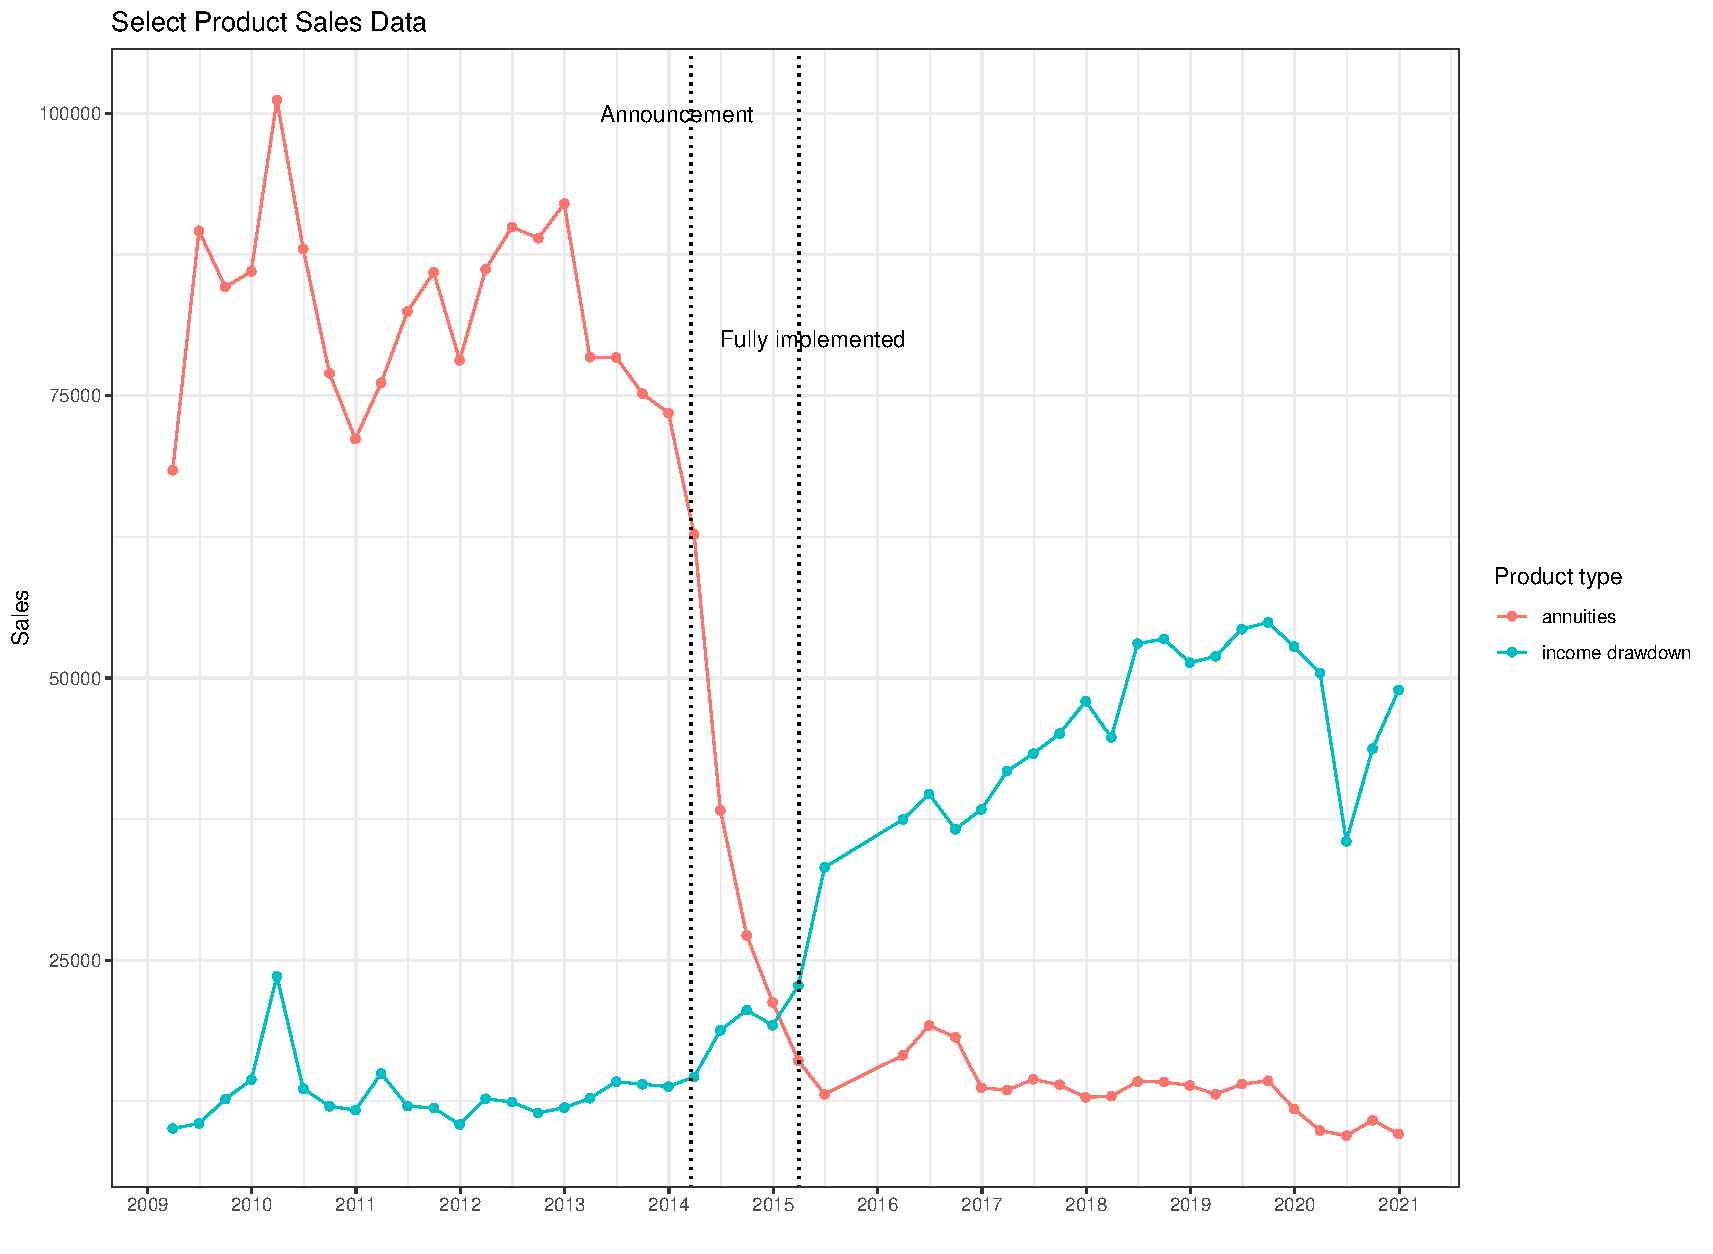
\includegraphics[width=0.9\columnwidth]{figures/annuity_overtime.pdf}

    \caption{Product Sales Data}
    \label{fig:annovertime}
\end{figure}

\begin{figure}[h]

    \centering
    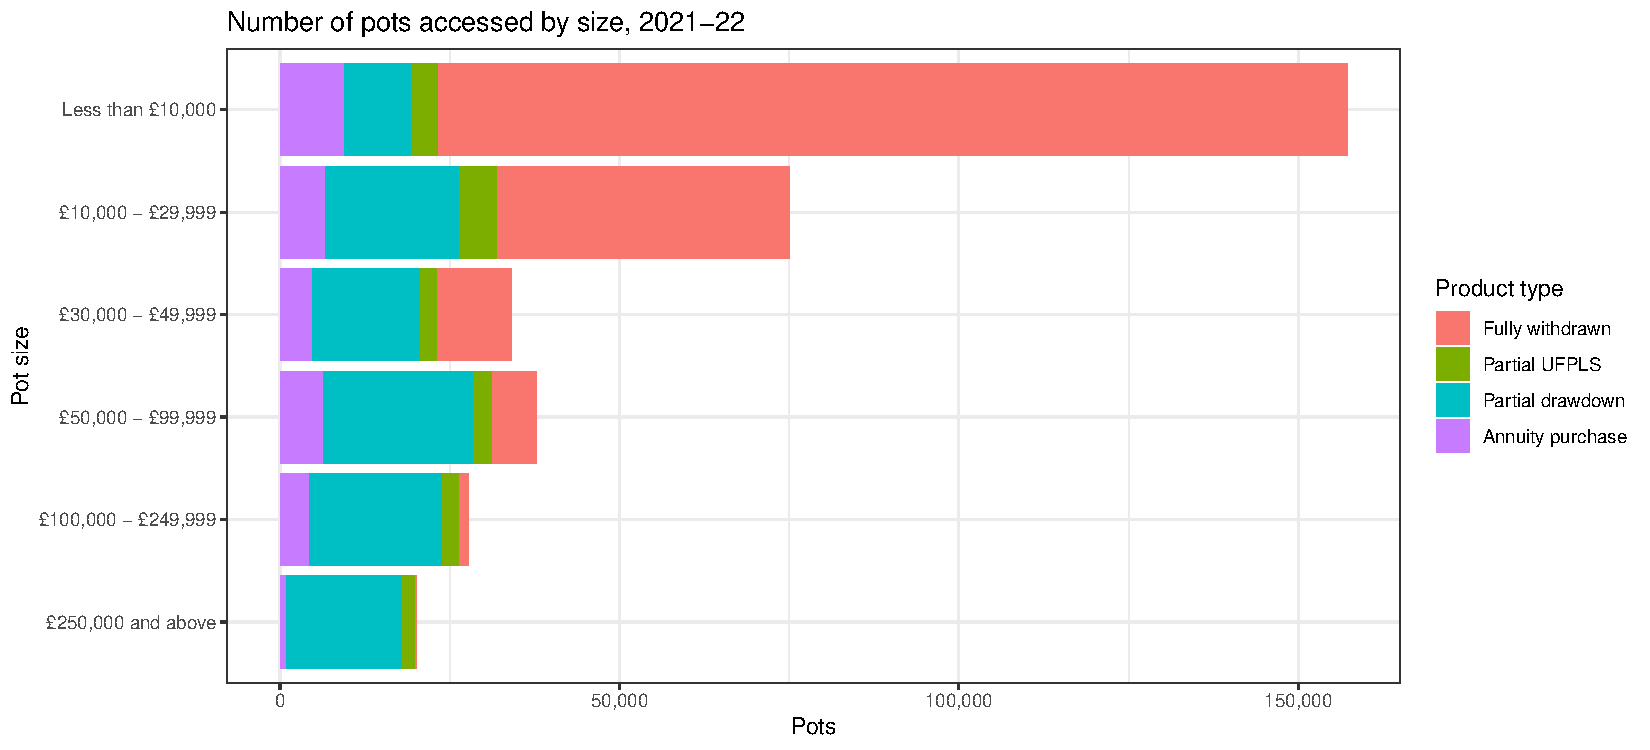
\includegraphics[width=0.9\columnwidth]{figures/annuity_pot_sizes.pdf}
    \caption[Caption for LOF]{How pension pots are accessed\protect\footnotemark}
    \label{fig:ann2122}

    \
\end{figure}
Figure \ref{fig:ann2122} shows the distribution of methods used to access pension pots
at retirement in 2021-22. In 2021, 196,736 pots were fully withdrawn at
retirement, accounting for over 50\% of pots. Prior to the policy reform this
was not the case -- most DC pension pots were accessed through
annuitisation.

Also of specific interest to the annuity market was the European Union's `Equal
Treatment in Goods and Services Directive' of 2004. This prohibited
discrimination in the provision and cost of goods and services based on sex. Up
until 2011, there was a clause that stated insurers were allowed to charge
different premiums if this was based on evidence that sex is correlated with
different amounts of risk. However, in March 2011, the European Court of Justice
ruled that insurers were not allowed to charge different amounts and gave them
until December 2012 to implement the ruling. This change meant that annuity
products could no longer be priced differently for men and women in the UK --
changing the money's worth of an annuity. I run a robustness test in the
empirical section to check whether this reform biases my results.

\footnotetext{Partial UFPLS (uncrystallised funds pension lump sum) is similar
    to Partial drawdown but with a different tax schedule. With partial drawdown
    you take the whole 25\% tax-free amount at once whereas with UFPLS you only
    claim the tax relief on 25\% of the amount you are taking out. This option
    is better if you may want to buy another retirement product in the future
    such as an annuity. }


\subsection{Covariate balance}

Table \ref{tab:sum_stats} shows various summary statistics for each variable of
interest from ELSA and the ONS.

An individual is defined as treated if they retired between and including 2015
and 2017, and an individual is in the control group if they retired in 2014 or
earlier. Since I am interested in consumption in early retirement, an
individuals interview date needs to be within the first three years of them
retiring.

The treated retirement group is smaller with just 303 non missing observations
for gender as opposed to 765 individuals in the control group. The control group
are more male, retired at a slightly younger age and expected to retire slightly
earlier. This could be because this period was affected by the increase in the
state pension age for women from age 60 in 2010 to age 65 in 2018, so early
cohorts had slightly earlier state pension eligibility ages. But, this change
happened gradually and ocurred over the whole period, so I do not expect it to
influence the results. The DifferenceAge row tracks the difference between
expected and actual retirement age.

The treatment group has higher financial wealth with a median of £67,000 at the
time of interview as opposed to £54,300 in the control group. Likewise, the
second group are more likely to have held a DC pension at some point and have
more money in them. Both groups are equally likely to have a DB pension with
roughly 45\% of individuals across both samples having a DB pension. In general,
DB pensions are more prevalent than DC pensions in the data -- this reflects the
trend that is observed in the general UK population. Home ownership is roughly
equal across groups although the second group has slightly higher housing
wealth.

Both groups are similarly long-lived when using ONS life tables to calculate
life expectancy based on gender, age and the year the interview was carried out
in. Subjective life expectancies are also similar across groups, with
individuals expecting to live another 21 years as opposed to the 24 that the ONS
would expect them to live.

Unfortunately, some consumption data is missing for some individuals. The food
categories have the least missing data and the leisure consumption category has
the most missing data.

Overall, the groups appear to have slightly different wealth profiles with the
treatment group being richer and slightly more likely to have DC pension wealth.
On key demographic characteristics, however, the groups are similar. The
difference in retirement age between the two groups can be mostly explained by
the difference in expected retirement age meaning that individuals have not en
masse decided to delay retirement and avoid annuitisation. Moreover, for the
regression discontinuity models I only use individuals who have a DC pension, so
it does not matter that there are more individuals with DC pensions in the
second group.

\begin{landscape}
    \linespread{1.25}
    \begin{table}

\caption{Summary statistics \label{tab:sum_stats} }
\centering
\fontsize{10}{12}\selectfont
\begin{tabular}[t]{lrrrrrrrrrr}
\toprule
\multicolumn{1}{c}{ } & \multicolumn{2}{c}{Max} & \multicolumn{2}{c}{Mean} & \multicolumn{2}{c}{Median} & \multicolumn{2}{c}{Min} & \multicolumn{2}{c}{Non Missing} \\
\cmidrule(l{3pt}r{3pt}){2-3} \cmidrule(l{3pt}r{3pt}){4-5} \cmidrule(l{3pt}r{3pt}){6-7} \cmidrule(l{3pt}r{3pt}){8-9} \cmidrule(l{3pt}r{3pt}){10-11}
 & Control & Treat & Control & Treat & Control & Treat & Control & Treat & Control & Treat\\
\midrule
Gender & 1.0 & 1.0 & 0.470 & 0.495 & 0.0 & 0.0 & 0.0 & 0.0 & 753 & 301\\
RetirementYear & 2013.0 & 2017.0 & 2011.875 & 2015.389 & 2012.0 & 2015.0 & 2011.0 & 2015.0 & 753 & 301\\
InterviewYear & 2016.0 & 2017.0 & 2013.328 & 2016.326 & 2014.0 & 2016.0 & 2011.0 & 2015.0 & 753 & 301\\
YearsSinceRetirement & 2.0 & 2.0 & 1.057 & 0.528 & 1.0 & 1.0 & 0.0 & 0.0 & 753 & 301\\
RetiredAge & 82.0 & 79.0 & 63.052 & 63.877 & 63.0 & 64.0 & 55.0 & 55.0 & 753 & 301\\
\addlinespace
AgeAtInterview & 83.0 & 79.0 & 64.109 & 64.405 & 64.0 & 64.0 & 55.0 & 55.0 & 753 & 301\\
ExpectedRetiredAge & 120.0 & 120.0 & 62.317 & 62.773 & 60.0 & 60.0 & 54.0 & 50.0 & 605 & 264\\
DifferenceAge & 48.0 & 44.0 & -0.660 & -0.981 & -1.0 & -1.0 & -8.0 & -22.0 & 605 & 264\\
FinWealth(£000s) & 1.9 & 2.0 & 0.122 & 0.168 & 0.1 & 0.1 & -0.0 & -0.0 & 738 & 297\\
DCPension & 1.0 & 1.0 & 0.198 & 0.259 & 0.0 & 0.0 & 0.0 & 0.0 & 753 & 301\\
\addlinespace
DCValue(£000s) & 8.2 & 17.3 & 0.073 & 0.116 & 0.0 & 0.0 & 0.0 & 0.0 & 684 & 259\\
DBPension & 1.0 & 1.0 & 0.466 & 0.455 & 0.0 & 0.0 & 0.0 & 0.0 & 753 & 301\\
StatePension & 0.0 & 0.0 & 0.005 & 0.005 & 0.0 & 0.0 & 0.0 & 0.0 & 750 & 298\\
OwnsHouse & 1.0 & 1.0 & 0.875 & 0.880 & 1.0 & 1.0 & 0.0 & 0.0 & 753 & 301\\
HouseValue(£000s) & 1.3 & 1.7 & 0.230 & 0.296 & 0.2 & 0.2 & 0.0 & -0.1 & 753 & 301\\
\addlinespace
ObjectiveLifeExp & 33.7 & 34.1 & 23.732 & 23.904 & 23.9 & 23.5 & 7.9 & 10.8 & 753 & 301\\
SubjectiveLifeExp & 36.6 & 37.9 & 20.898 & 20.950 & 21.3 & 21.2 & 4.6 & 5.3 & 527 & 198\\
TotalConsump & 2925.1 & 3495.7 & 729.239 & 780.975 & 647.6 & 699.5 & 130.2 & 136.9 & 753 & 301\\
FoodConsump & 1938.1 & 1938.1 & 415.753 & 425.780 & 363.3 & 373.8 & 51.5 & 36.1 & 748 & 296\\
FoodConsumpIn & 440.0 & 400.0 & 79.964 & 77.706 & 70.0 & 70.0 & 10.0 & 1.0 & 749 & 296\\
\addlinespace
FoodConsumpOut & 750.0 & 1200.0 & 68.302 & 88.208 & 50.0 & 50.0 & 0.0 & 0.0 & 752 & 298\\
ClothingConsump & 1450.0 & 2000.0 & 89.224 & 83.824 & 45.0 & 40.0 & 0.0 & 0.0 & 753 & 301\\
LeisureConsump & 530.0 & 150.0 & 82.072 & 75.000 & 60.0 & 75.0 & 0.0 & 0.0 & 657 & 2\\
UtilityConsump & 483.1 & 580.9 & 107.840 & 113.324 & 96.0 & 100.0 & 0.0 & 0.0 & 753 & 301\\
\bottomrule
\end{tabular}
\end{table}

    \normalsize
\end{landscape}


As a further test for balance I regress demographic and financial
characteristics of individuals on the treatment dummy. We can then see if the
treatment and control groups differ on key characteristics such as financial
wealth or retirement age. For a regression discontinuity to be valid we need the
groups to be similar along all other characteristics apart from the treatment
variable.

In particular I run:
\begin{equation*}
    Y_{i} = \alpha + \beta PostRef_{i}  + \epsilon_{i}
\end{equation*}

Where $Y_{i}$ are the different demographic and financial characteristics for
only those individuals with a DC pension.

\linespread{1}
\begin{table}

\caption{Covariate Balance \label{tab:cov_balance}}
\centering
\begin{tabular}[t]{lll}
\toprule
 & Pt. est. & SE\\
\midrule
Gender & 2.243 & 10.468\\
RetirementYear & -12.528 & 16.127\\
InterviewYear & -11.243 & 24.959\\
YearsSinceRetirement & 9.716 & 16.056\\
RetiredAge & -12.528 & 16.127\\
\addlinespace
ExpectedRetiredAge & -240.427 & 129.345\\
DifferenceAge & -246.763 & 128.979\\
FinancialWealth (thousands) & -4769.638 & 5410.054\\
DCPension & -13.608 & 8.933\\
DCValue (thousands) & -1978.144 & 20284.768\\
\addlinespace
DBPension & 7.974 & 10.386\\
OwnsHouse & -0.697 & 6.968\\
HouseValue (thousands) & 6630.186 & 4775.236\\
ObjectiveLifeExp & 13.086 & 30.559\\
SubjectiveLifeExp & 0.351 & 182.705\\
\bottomrule
\end{tabular}
\end{table}

\linespread{1.5}

Table \ref{tab:cov_balance} shows these results. As expected, retirement year
and interview year are greater for the treated group. The difference between
expected and real retirement age is 0, which shows that individuals are not
delaying retirement, beyond their original expectation, in order to be part of
the treatment. DC pension value is higher, as is financial wealth but these are
both imprecisely estimated. Because of the differences in these variables I add
them to the regression model.

One threat to validity is manipulation of the running variable, retirement year.
As observed above in Tables \ref{tab:sum_stats} and \ref{tab:cov_balance}, it
does not appear as though individuals are delaying retirement. However, it is
possible that individuals do not buy an annuity at the time of retirement since
the law prior to 2014 only required that they access the pot by age 75. They may
decide to keep their DC pension untouched and live off other income and assets
before accessing it later. Since I do not have data for when individuals
purchase annuities, I cannot track whether annuity purchases were delayed for
people in the treatment group. However, there is relatively stable annuity
demand before the policy
reform. If individuals delayed annuity purchases in expectation of the reform,
so that they would not have to buy an annuity at all, we would observe declines
in purchases before the reform was announced. Likewise, if individuals bought an
annuity early in expectation that the end of the compulsory market would cause
prices to go up, we would observe a spike in annuity purchases prior to 2014.

Moreover, if individuals retired and then delayed purchasing an annuity, the
control group would have lower rates of annuitisation as well. This would bias
my results downward, since then individuals who retired in prior to the policy
change would also be consuming more.


\section{Empirical models}

In this section, I outline the key empirical models I run, first with real
data from ELSA, and then with simulated data from the lifecycle models. I then
see which lifecycle model better fits the consumption response that occurred as
a result of the pension reform.

I use a fuzzy regression discontinuity design for which I compare the
consumption of individuals who retired after the policy reform to that of people
who retired just before the reform. The key assumption implicit in regression
discontinuities is that nothing else changes at the time of the jump apart from
the policy of interest, and that the policy occurs without individuals
predicting it and altering their behaviour. As I have argued above, the
demographic information in the data suggests that individuals did not delay
retirement and that there was no delay in annuitisation as shown by the quick
and sudden decline in annuity purchases. Moreover, anecdotal evidence from media
and business sources at the time of the announcement show that there was
surprise the government put forward the reform, with Money Marketing describing
the change as a ``bombshell" \citep{money_marketing_announcement}.

I use consumption data of individuals up to 3 years into their retirement so
that the sample size is larger. So, if someone retired in 2015 and had
consumption data in 2015 and 2017, I include both values.

Because of the differences in financial characteristics between the groups, I
add controls for financial wealth, housing wealth, whether an individual owns
their own home, their gender and the size of their state pension. The following
regression equation is used.

\begin{equation*}
    Cons_{it} =  \gamma X_{it} + \beta PostReform_{it} + \epsilon
\end{equation*}

Where $Cons_{it}$ is one of five different consumption variables and $X_{it}$ is
a set of controls.

Table \ref{tab:DcOnlyRes} shows the results of this specification on the various
consumption indicators. Column 1 has total monthly consumption on the left hand
side of the regression equation. We can see that being in the treatment group is
associated with £36 more a week in spending overall. This is statistically
significant using robust standard errors clustered at the treatment level. Being
further into retirement at the time of interview is associated with higher total
consumption -- this is surprising since lifecycle models predict consumption
decreases over retirement and this has also been documented empirically
\citep{hurd_rohwedder_nber_2003}.

Columns 2 through 4 use food consumption as the outcome variable. Interestingly,
food consumption inside the house does not increase as a result of the policy
reform but food consumed away from the house does increase. A shock to income,
caused by no longer needing to annuitise, may cause spending on luxury goods to
increase and for spending on their substitutes, like food in the house relative
to food away from home, to decrease. This wealth effect may be driving the
results we observe in Table \ref{tab:DcOnlyRes}, since food consumption outside the
home increases as does expenditure on clothing -- seen in column 5.

One concern is that the group who retired after 2014 are just generally
different to those who retired before and perhaps consume more outside the home
anyway. The financial characteristic data presented in Table \ref{tab:sum_stats}
would support this hypothesis as it shows all retirees are richer post-reform.
To test for these cohort effects, I run a difference-in-difference (DD)
regression to complement the regression discontinuity just shown. I add
individuals who have a DB pension and those with no private pension into the
model and interact the policy change with dummies for having different types of
pension. Specifically, I run:

\begin{equation*}
    Cons_{it} =  \gamma X_{it} + \beta_{1} PostReform_{it} + \beta_{2} PostReform*DC_{it} + \beta_{3} PostReform*DB_{it}  + \epsilon
\end{equation*}


This makes the coefficient of interest $\beta_{2}$, which shows us the
difference in the change in consumption between the DC-only group and the base
group that has neither a DB or DC pension. Since rules for DB pensions did not
change under the pensions freedom act, those with a DB pension or no pension can
be seen as a natural counterfactual group to judge the consumption of the DC
group against.

The key identifying assumption for DD is the parallel trends assumption. In this
context, it means that consumption differences between the DB, DC and no pension
groups across cohorts would have been the same were it not for the policy change.
Therefore, for DD to be invalid, we would need a reason to expect that the
individuals with a DB and no pension who are retiring post-2014 are impacted by
some factor that did not equally impact the DC group. Given that there were no
other pension reforms at this time that differently affected these groups, I
claim that the parallel trends assumption holds.

Table \ref{tab:ElsaAllData} shows these results. The interactions at the bottom
of the table show us what happened to individuals with a given pension type
relative to the reference cohort, which has no pension. Those with only a DC
pension had an increase in total consumption which was higher than those with a
DB pension and higher than those with no pension. Consumption on food decreased
slightly for the DC group relative to no pension, but the decrease was less than
that for the DB group. Expenditure on clothing increased for the DC group
relative to the no pension and DB pension groups. The increase in sample size
also brings decreases in the standard errors of these variables -- the
interactions are now all significant a the 5\% level as is the main coefficient
on retiring post-reform.

However, it is worth noting that there is a significant change between the DB
and the no pension group. A natural test of the parallel trends assumption is to
see whether two different, untreated, units have different outcomes
post-treatment. If they are different post treatment then there could be
something else driving the differences between the treatment group and the
non-treated groups. This therefore raises questions about the validity of the DD
regression in this setting.

We can also test whether treatment intensity is correlated with larger increases
in spending. Those who have more money in a DC pension would be impacted by the
policy to a greater extent than those with smaller pensions, since they would be
forced to annuitise a larger amount. So, I interact the policy with DC wealth.
As in Table \ref{tab:DcOnlyRes}, this regression only uses those individuals who
have a DC pension.

Specifically, I run:
\begin{equation*}
    Cons_{it} =  \gamma X_{it} + \beta PostReform_{it}*DCValue_{it} + \epsilon_{it}
\end{equation*}

Table \ref{tab:DcOnlyInteract} shows the results. The interaction with DC
pension size is positive, meaning that a larger DC pension pot is associated with a
greater increase in total monthly consumption. For the all other categories,
more pension wealth is associated with lower consumption, though for food out
the house and for clothing the main coefficients are still positive and
significant.

As mentioned above, the DC pension pot value data after
wave 5 has not been released yet, so for individuals who retire after 2011 I
have no DC wealth variable. For Table \ref{tab:DcOnlyInteract}, pension wealth
from the last available year for an individual was given a real return of 3\%
and compounded until year of interview. Given that this is an imperfect measure,
I also run the regression with financial wealth interacted with the treatment
variable.

Table \ref{tab:DcOnlyFinWealthInteract} contains these results and shows a
similar pattern to Table \ref{tab:DcOnlyInteract}. The reform is associated with
an increase in total monthly consumption and more financial wealth increases the
size of this effect. As for the DC pension value variable, the interactions
in the regressions of the other consumption variables have negative signs.

\begin{landscape}
    \linespread{1}
    \begin{table}

\caption{DC Only \label{tab:DcOnlyRes}}
\centering
\begin{tabular}[t]{lddddd}
\toprule
  & {TotalConsump} & {FoodConsump} & {FoodConsumpIn} & {FoodConsumpOut} & {ClothingConsump}\\
\midrule
(Intercept) & 1021.473 & 336.236 & 51.012 & 111.948 & -40.948\\
 & (311.124) & (88.870) & (37.892) & (76.345) & (288.889)\\
PostReform & -263.566 & 28.985 & 18.670 & -49.062 & -51.413\\
 & (16.736) & (8.018) & (5.111) & (13.483) & (34.475)\\
rv & 81.454 & -5.037 & -4.324 & 13.410 & -8.369\\
 & (2.204) & (1.906) & (0.365) & (3.358) & (3.877)\\
RetiredAge & 0.668 & 0.215 & 0.126 & -0.314 & 0.635\\
 & (5.180) & (1.061) & (0.641) & (1.734) & (4.967)\\
FinWealth(£000s) & 0.245 & 0.143 & 0.006 & 0.108 & -0.019\\
 & (0.122) & (0.015) & (0.002) & (0.014) & (0.030)\\
Gender & -39.881 & -34.203 & -8.601 & 2.464 & 10.879\\
 & (34.523) & (14.191) & (1.892) & (20.927) & (36.216)\\
DCValue(£000s) & -0.016 & 0.006 & 0.002 & -0.004 & -0.006\\
 & (0.006) & (0.007) & (0.001) & (0.003) & (0.002)\\
YearsSinceRetirement & 27.491 & -7.975 & -1.441 & -2.648 & 12.890\\
 & (20.390) & (8.144) & (2.536) & (2.633) & (5.426)\\
OwnsHouse & -115.386 & 118.737 & 25.877 & 7.199 & 81.823\\
 & (18.262) & (38.551) & (0.648) & (40.684) & (6.002)\\
StatePension & -12.412 & -4.698 & -0.915 & -0.497 & -3.962\\
 & (2.809) & (2.929) & (0.876) & (0.709) & (7.634)\\
PostReform:rv & 10.776 & -11.726 & -4.714 & 8.585 & 80.550\\
 & (16.406) & (13.998) & (2.851) & (1.129) & (11.147)\\
\midrule
Num.Obs. & 208 & 205 & 205 & 208 & 208\\
R2 & 0.071 & 0.061 & 0.057 & 0.106 & 0.053\\
R2 Adj. & 0.023 & 0.013 & 0.008 & 0.060 & 0.005\\
\bottomrule
\multicolumn{6}{l}{\rule{0pt}{1em}I use robust standard errors clustered at the treatment level
    since standard errors are
    likely correlated within these groups.}\\
\end{tabular}
\end{table}

\end{landscape}

\begin{landscape}
    \linespread{1}
    \begin{table}

\caption{All individuals with interaction \label{tab:ElsaAllData}}
\centering
\begin{tabular}[t]{lddddd}
\toprule
  & {TotalConsump} & {FoodConsump} & {FoodConsumpIn} & {FoodConsumpOut} & {ClothingConsump}\\
\midrule
(Intercept) & 588.449 & 376.400 & 81.643 & 23.591 & 129.552\\
 & (140.286) & (31.367) & (12.656) & (85.192) & (35.146)\\
PostReform & 94.121 & 14.164 & -1.591 & 21.122 & -1.439\\
 & (4.541) & (0.419) & (0.335) & (1.215) & (0.657)\\
DCPension & 48.471 & 29.337 & 3.056 & 15.300 & -3.224\\
 & (4.408) & (2.544) & (0.503) & (0.260) & (1.616)\\
DBPension & 90.885 & 16.998 & -0.356 & 18.744 & 22.568\\
 & (2.243) & (5.906) & (0.190) & (5.217) & (1.797)\\
RetiredAge & 2.320 & -0.781 & -0.218 & 0.140 & -1.609\\
 & (2.643) & (0.136) & (0.272) & (1.301) & (0.867)\\
FinWealth(£000s) & 0.166 & 0.072 & -0.002 & 0.080 & 0.017\\
 & (0.009) & (0.028) & (0.006) & (0.005) & (0.013)\\
Gender & -19.453 & -19.704 & -5.024 & 2.024 & -0.014\\
 & (9.136) & (26.358) & (4.913) & (4.729) & (2.243)\\
DCValue(£000s) & -0.012 & 0.004 & 0.002 & -0.003 & -0.004\\
 & (0.000) & (0.009) & (0.002) & (0.002) & (0.002)\\
YearsSinceRetirement & 37.784 & -10.041 & -2.018 & -1.564 & 6.843\\
 & (10.397) & (0.877) & (0.992) & (3.449) & (1.411)\\
OwnsHouse & -90.415 & 110.119 & 20.541 & 20.923 & 42.791\\
 & (27.860) & (2.329) & (2.187) & (7.207) & (5.948)\\
StatePension & -5.971 & -2.925 & -0.445 & -0.957 & 0.669\\
 & (3.949) & (2.058) & (0.416) & (0.269) & (2.020)\\
PostReform:DCPension & 12.823 & -4.930 & -0.463 & -2.085 & 37.406\\
 & (3.134) & (0.311) & (0.172) & (0.262) & (0.411)\\
PostReform:DBPension & -139.946 & -24.437 & -1.744 & -16.814 & -15.134\\
 & (2.228) & (0.024) & (0.290) & (1.385) & (0.565)\\
\midrule
Num.Obs. & 926 & 917 & 918 & 923 & 926\\
R2 & 0.039 & 0.049 & 0.031 & 0.105 & 0.029\\
R2 Adj. & 0.027 & 0.036 & 0.018 & 0.093 & 0.016\\
\bottomrule
\multicolumn{6}{l}{\rule{0pt}{1em}I use robust standard errors clustered at the treatment level
    since standard errors are
    likely correlated within these groups.}\\
\end{tabular}
\end{table}

\end{landscape}
\begin{landscape}
    \linespread{1}
    \begin{table}

\caption{DC Pension Size interaction \label{tab:DcOnlyInteract}}
\centering
\begin{tabular}[t]{lccccc}
\toprule
  & TotalConsump & FoodConsump & FoodConsumpIn & FoodConsumpOut & ClothingConsump\\
\midrule
(Intercept) & \num{1347.198} & \num{571.090} & \num{77.009} & \num{220.315} & \num{40.944}\\
 & (\num{745.238}) & (\num{346.747}) & (\num{68.914}) & (\num{122.712}) & (\num{217.875})\\
PostReform & \num{74.604} & \num{9.797} & \num{0.123} & \num{11.064} & \num{27.427}\\
 & (\num{69.978}) & (\num{27.205}) & (\num{5.366}) & (\num{9.226}) & (\num{24.871})\\
RetiredAge & \num{-4.652} & \num{-3.172} & \num{-0.073} & \num{-2.585} & \num{-0.295}\\
 & (\num{10.447}) & (\num{5.435}) & (\num{1.089}) & (\num{1.893}) & (\num{3.609})\\
FinancialWealth (thousands) & \num{0.229} & \num{0.172} & \num{0.013} & \num{0.111} & \num{-0.012}\\
 & (\num{0.114}) & (\num{0.050}) & (\num{0.010}) & (\num{0.025}) & (\num{0.053})\\
Gender & \num{-19.457} & \num{-35.355} & \num{-6.937} & \num{-6.007} & \num{13.359}\\
 & (\num{63.228}) & (\num{28.103}) & (\num{5.502}) & (\num{10.149}) & (\num{24.880})\\
DCValue (thousands) & \num{-0.009} & \num{0.022} & \num{0.006} & \num{-0.004} & \num{-0.002}\\
 & (\num{0.027}) & (\num{0.035}) & (\num{0.008}) & (\num{0.004}) & (\num{0.009})\\
YearsSinceRetirement & \num{-1.902} & \num{-7.906} & \num{-0.268} & \num{-7.741} & \num{6.092}\\
 & (\num{44.666}) & (\num{16.767}) & (\num{3.225}) & (\num{6.186}) & (\num{14.714})\\
OwnsHouse & \num{-261.541} & \num{101.085} & \num{20.990} & \num{10.656} & \num{73.604}\\
 & (\num{196.144}) & (\num{37.911}) & (\num{7.293}) & (\num{14.787}) & (\num{16.328})\\
StatePension & \num{-14.040} & \num{-4.125} & \num{-1.256} & \num{1.258} & \num{-3.040}\\
 & (\num{9.566}) & (\num{4.105}) & (\num{0.841}) & (\num{1.265}) & (\num{4.052})\\
PostReform:DCValue (thousands) & \num{-0.003} & \num{-0.022} & \num{-0.005} & \num{0.000} & \num{-0.002}\\
 & (\num{0.045}) & (\num{0.035}) & (\num{0.008}) & (\num{0.004}) & (\num{0.017})\\
\midrule
Num.Obs. & \num{209} & \num{326} & \num{326} & \num{330} & \num{221}\\
R2 & \num{0.068} & \num{0.066} & \num{0.051} & \num{0.102} & \num{0.035}\\
R2 Adj. & \num{0.026} & \num{0.039} & \num{0.024} & \num{0.076} & \num{-0.006}\\
AIC & \num{3156.1} & \num{4500.7} & \num{3452.4} & \num{3836.7} & \num{2897.0}\\
BIC & \num{3192.9} & \num{4542.4} & \num{3494.1} & \num{3878.5} & \num{2934.4}\\
Log.Lik. & \num{-1567.065} & \num{-2239.361} & \num{-1715.225} & \num{-1907.357} & \num{-1437.504}\\
RMSE & \num{436.58} & \num{232.82} & \num{46.64} & \num{78.33} & \num{161.68}\\
Std.Errors & HC3 & HC3 & HC3 & HC3 & HC3\\
\bottomrule
\end{tabular}
\end{table}

\end{landscape}

\begin{landscape}
    \linespread{1}
    \begin{table}

\caption{DC Financial Wealth interaction \label{tab:DcOnlyFinWealthInteract}}
\centering
\begin{tabular}[t]{lddddd}
\toprule
  & {TotalConsump} & {FoodConsump} & {FoodConsumpIn} & {FoodConsumpOut} & {ClothingConsump}\\
\midrule
(Intercept) & 792.453 & 157.868 & 56.231 & -89.273 & 110.932\\
 & (380.887) & (479.454) & (55.927) & (238.508) & (241.514)\\
PostReform & 77.996 & 9.980 & -2.599 & 20.981 & 30.043\\
 & (3.083) & (6.929) & (0.644) & (9.406) & (8.346)\\
RetiredAge & 2.134 & 4.024 & 0.201 & 3.187 & -1.370\\
 & (3.940) & (8.389) & (0.919) & (4.432) & (4.258)\\
FinWealth(£000s) & 0.322 & 0.164 & 0.009 & 0.117 & 0.059\\
 & (0.068) & (0.001) & (0.003) & (0.011) & (0.026)\\
Gender & -31.169 & -47.768 & -8.490 & -11.772 & 8.354\\
 & (33.636) & (21.976) & (2.569) & (31.747) & (32.934)\\
YearsSinceRetirement & 0.541 & -23.842 & -2.771 & -12.460 & -11.846\\
 & (8.561) & (1.625) & (4.359) & (16.759) & (4.174)\\
OwnsHouse & -139.190 & 102.073 & 25.433 & -8.030 & 74.816\\
 & (121.783) & (6.659) & (2.061) & (2.063) & (1.233)\\
StatePension & -15.442 & -7.971 & -0.775 & -4.373 & -0.596\\
 & (9.403) & (7.492) & (1.175) & (2.615) & (7.285)\\
PostReform:FinWealth(£000s) & 0.098 & -0.025 & -0.003 & -0.002 & -0.116\\
 & (0.064) & (0.015) & (0.001) & (0.015) & (0.030)\\
\midrule
Num.Obs. & 222 & 219 & 219 & 222 & 222\\
R2 & 0.077 & 0.072 & 0.048 & 0.088 & 0.030\\
R2 Adj. & 0.042 & 0.037 & 0.012 & 0.054 & -0.007\\
\bottomrule
\multicolumn{6}{l}{\rule{0pt}{1em}I use robust standard errors clustered at the treatment level
    since standard errors are
    likely correlated within these groups.}\\
\end{tabular}
\end{table}

\end{landscape}
\begin{landscape}
    \linespread{1}
    \begin{table}

\caption{Robustness: DC only and retire in year expected  \label{tab:DcOnlyExpOnlyRes}}
\centering
\begin{tabular}[t]{lddddd}
\toprule
  & {TotalConsump} & {FoodConsump} & {FoodConsumpIn} & {FoodConsumpOut} & {ClothingConsump}\\
\midrule
(Intercept) & 223.328 & 228.152 & 16.780 & 155.238 & 379.560\\
 & (718.134) & (418.206) & (36.356) & (260.230) & (280.871)\\
PostReform & -85.132 & -13.556 & -0.221 & -12.597 & 18.688\\
 & (36.067) & (35.093) & (4.856) & (13.994) & (5.473)\\
RetiredAge & 12.738 & 1.438 & 0.685 & -1.538 & -5.667\\
 & (12.368) & (7.840) & (0.779) & (4.456) & (4.088)\\
FinWealth(£000s) & 0.020 & -0.111 & -0.039 & 0.058 & -0.065\\
 & (0.040) & (0.215) & (0.022) & (0.121) & (0.195)\\
Gender & -43.490 & -7.026 & -2.946 & 5.777 & -32.277\\
 & (80.291) & (77.202) & (14.379) & (14.723) & (13.827)\\
DCValue(£000s) & -0.064 & 0.018 & 0.008 & -0.015 & -0.018\\
 & (0.001) & (0.031) & (0.006) & (0.006) & (0.017)\\
YearsSinceRetirement & 7.220 & 3.169 & -1.952 & 11.651 & 0.371\\
 & (70.654) & (42.979) & (6.381) & (15.251) & (7.456)\\
OwnsHouse & -61.528 & 152.220 & 31.645 & 14.714 & 74.843\\
 & (62.367) & (72.091) & (11.458) & (22.301) & (12.059)\\
StatePension & -39.402 & -8.484 & -1.134 & -3.555 & -0.388\\
 & (1.804) & (5.496) & (1.132) & (0.578) & (4.111)\\
\midrule
Num.Obs. & 65 & 65 & 65 & 65 & 65\\
R2 & 0.183 & 0.092 & 0.093 & 0.135 & 0.127\\
R2 Adj. & 0.066 & -0.038 & -0.037 & 0.011 & 0.002\\
\bottomrule
\multicolumn{6}{l}{\rule{0pt}{1em}I use robust standard errors clustered at the treatment level
    since standard errors are
    likely correlated within these groups.}\\
\end{tabular}
\end{table}

\end{landscape}

\begin{landscape}
    \linespread{1}
    \begin{table}

\caption{Robustness: DC only and retired later than 2012 \label{tab:DcOnlyNot2012}}
\centering
\begin{tabular}[t]{lddddd}
\toprule
  & {TotalConsump} & {FoodConsump} & {FoodConsumpIn} & {FoodConsumpOut} & {ClothingConsump}\\
\midrule
(Intercept) & 1524.689 & 207.316 & -0.021 & 206.030 & -77.148\\
 & (602.488) & (78.332) & (35.665) & (69.557) & (66.097)\\
PostReform & -129.407 & -0.283 & 3.941 & -17.300 & 26.287\\
 & (45.616) & (5.313) & (0.269) & (4.585) & (16.931)\\
RetiredAge & -6.681 & 1.996 & 0.987 & -2.276 & 2.379\\
 & (11.222) & (1.139) & (0.537) & (1.100) & (1.274)\\
FinWealth(£000s) & 0.051 & 0.142 & 0.012 & 0.089 & -0.047\\
 & (0.061) & (0.018) & (0.004) & (0.000) & (0.033)\\
Gender & 63.550 & -14.860 & -3.892 & 2.186 & 31.105\\
 & (92.963) & (52.718) & (2.789) & (39.938) & (23.118)\\
DCValue(£000s) & -0.010 & 0.000 & 0.001 & -0.006 & -0.002\\
 & (0.002) & (0.001) & (0.001) & (0.001) & (0.001)\\
YearsSinceRetirement & -48.503 & 13.926 & 6.890 & -15.919 & -17.179\\
 & (78.693) & (2.126) & (1.381) & (7.674) & (26.821)\\
OwnsHouse & -161.994 & 110.350 & 16.508 & 38.709 & 61.227\\
 & (96.075) & (82.579) & (11.563) & (32.757) & (30.533)\\
StatePension & -7.413 & -2.976 & -1.191 & 2.201 & -8.844\\
 & (4.752) & (8.688) & (1.654) & (1.490) & (3.568)\\
\midrule
Num.Obs. & 104 & 103 & 103 & 104 & 104\\
R2 & 0.049 & 0.049 & 0.042 & 0.075 & 0.053\\
R2 Adj. & -0.031 & -0.032 & -0.040 & -0.003 & -0.027\\
\bottomrule
\multicolumn{6}{l}{\rule{0pt}{1em}I use robust standard errors clustered at the treatment level
    since standard errors are
    likely correlated within these groups.}\\
\end{tabular}
\end{table}

\end{landscape}

\subsection{Robustness checks}

I carry out two checks for robustness. Firstly, I exclude those individuals who
retired more than one year away from their expected retirement year -- I define
an individual's expected retirement year as their expected retirement age in
their first interview with ELSA, added to the year that the interview was
carried out in. This checks whether the effects shown above are being driven by
individuals either retiring early in order to buy an annuity, since one may be
cheaper pre-reform because the compulsory market reduces adverse selection
\cite{finkelstein_porteba_2002}, or retiring later to avoid annuitisation
altogether.

I also check whether the EU reform to annuity pricing is changing the results in
some way. Since the reform only came into effect in December 2012, there are some
retirees in the sample who may have purchased an annuity before
annuity pricing was made the same for men and women. I drop anyone with a
retirement year in 2012 or 2011 and repeat the analysis from Table
\ref{tab:DcOnlyRes}.

Tables \ref{tab:DcOnlyExpOnlyRes} and \ref{tab:DcOnlyNot2012} show these
results. In Table \ref{tab:DcOnlyExpOnlyRes}, we see that the sign is reversed on
PostReform in all consumption categories apart from clothing, however the sample
size is a third of what it was prior to excluding individuals so there is more
uncertainty in these estimates. In Table \ref{tab:DcOnlyNot2012}, the sample
size is again much smaller and the sign has flipped on all consumption
categories apart from clothing and food consumed in the house. These regressions
show that there are potentially identification issues with the regression
discontinuity and DD strategies that I have presented thus far. However, since
the sample sizes for both the robustness tests and main results are small it is
difficult to assess what the true impact of the reform was.

In a third set of robustness checks, I would have varied which years of
retirement I assign to treatment or not, and varied the years of retirement that
I collect consumption data for. But, due to space constraints I do not present
these. The consumption response should diminish the longer the retirement year
period either side of 2014 that we take data from, and we should not see
positive results if we pick a `fake' treatment year, such as 2009, and run the
same set of regressions using this year.

In conclusion, the main results tables show that the reform could have had a
positive impact on consumption in early retirement, and this increase is clearer
for more `luxury' consumption goods, such as expenditure on clothing and eating
out. And, when we interact with a proxy for treatment strength (financial wealth
or pension size) the impact of the policy is larger the stronger the treatment.
However, the robustness checks point in the other direction, and there are
significant differences between the DB and no pension groups in the DD
regression, perhaps highlighting that other, unobserved, variables are driving
changes in consumption. For example, consumer confidence between years could be
changing, or, because of the small sample size in the ELSA dataset, there is too
much noise in the consumption values each year.

Theoretically, a null or small change in consumption is evidence for a
bequest motive explaining a lack of annuitisation rather than pessimistic life
expectancies being the cause. In the next section, I solve and simulate a
lifecycle model for individuals in the ELSA dataset. I find that the bequest
motive most closely matches the patterns observed in the empirical models above.

\section{Lifecycle theory}

In the second part of the paper, I first solve a modified retirement lifecycle
model, then simulate the ELSA data and run the empirical models from
above on the implied consumption data.

In recursive form, the problem that retirees face is as follows. Every period
retirees solve:
\begin{equation*}
    \underset{a_{t+1}, c_{t}}{\max} \{ u(c_{t}) + p_{t}B(a_{t+1}) + \beta(1-p_{t})V(a_{t+1}, y, t+1) \}
\end{equation*}
Where the maximised value of this objective function is denoted: $V(a_{t}, y,
    t)$. This is what I refer to as an individuals value function.
This is maximised subject to their budget constraint:
\begin{equation*}
    c_{t} =a_{t}(1 +r) -  a_{t+1} + y
\end{equation*}

where $a_{t}$ are asset holdings in time t, $y$ is constant income for all
periods, $p_{t}$ is probability of death in period $t$ conditional on being
alive at the start of the period. And $B()$ is a bequest function. Income comes
from the state pension and purchased annuities. I follow the literature and use
$\beta = 0.97$ as an individual's discount rate and $r = 1/0.97$ as the interest
rate. I enter $t$ directly into the value function as a state variable to make
it clear that value is also conditional on age -- through the chance of death
and the total number of periods left until terminal age.

Solving the value function gives us two `policy functions': $a_{t+1}(a_{t},
    y,t)$ for assets, and $c_{t}(a_{t}, y, t)$ for consumption. Policy
functions are functions of the state variables that maximise the value function.

As is common in the literature \citep{lockwood_red_2012,de_nardi_et_al_2010}, I
use a constant relative risk aversion utility function.
\begin{equation*}
    u(c_{t}) = \frac{c_{t}^{1 - \sigma}}{1 - \sigma}
\end{equation*}

Where $\sigma = 2.5$ which is around the median found in the retirement savings
literature.

In some specifications retirees can leave bequests. I use the bequest function
from \cite{lockwood_red_2012,lockwood_aer_2018}.
\begin{equation*}
    B(a_{t+1}) = \bigl( \frac{m}{1 - m} \bigr)^{\sigma}  \frac{(\frac{m}{1 - m}c_{0} + a_{t+1})^{(1 - \sigma)}}{1 - \sigma}
\end{equation*}

Where $a_{t+1}$ is the amount left at death. $c_{0}$ is the amount of
consumption below which individuals will not leave bequests. If $c_{0} >0$, then
bequests are a luxury good and the wealthier the individual the more they will
bequest. $m$ is the marginal propensity to bequeath after consuming at least
$c_{0}$, and a higher value of $m$ means that individuals will leave a greater
share of wealth to their heirs. I pick values of $m = 0.95$ and $c_{0} = \pounds
    20,000$ since these generate low rates of annuitisation. For comparison,
\cite{lockwood_aer_2018} finds $c_{0}$ is in the range of $\$12,000$ to
$\$30,000$ and $m$ is between $0.93$ and $0.96$ in a variety of estimated
models.

To solve this problem, I first discretise the state space. I create a grid from £500
to £50,000 incrementing by £500 for income and £1,000 to £500,000 incrementing
by £1,000 for financial assets. I solve the retirees' problem using backward
induction. At age 110, there is certainty of death so any leftover assets are
bequested. This means that the value of any remaining assets at age 111 is either 0 (if we do
not allow a bequest motive) or the value of bequests. I then take this value
function and solve an individual's problem at age 110, choosing assets for next
period (i.e. those to bequest) and how much to consume. This will be all assets
for individuals with no bequest motive or with assets below £20,000 ($c_{0}$).

Using the policy function at age 110, which we just found by doing the
optimisation at age 110, I calculate the value for all income and asset states
at age 110. This value is then used to solve the problem an individual at age
109 faces. Specifically, for each income and asset state, they need to find the
assets next period that maximise: utility from consumption; bequests multiplied
by the probability of death; and the value function at age 110, discounted by
$\beta$, multiplied by the probability of being alive. I repeat this process
back to the age of retirement to obtain optimal consumption amounts for each
year of retirement and the associated value functions. I write code in Julia
that solves this maximisation problem.

To simulate the ELSA data, I solve this retirement problem for each new retiree
in the dataset. I solve the problem with subjective and objective life
expectancies, and with and without a bequest motive.

In a retiree's first year of retirement, I sometimes annuitise a portion of
their wealth. In practical terms, this is moving down the asset grid but up the
permanent income grid. To assess this trade-off I calculate the annual annuity
payment that follows from a given annuity cost. I calculate this, using
objective life tables from the ONS, with the following equation:


\begin{equation*}
    Ann = \delta * C * \biggl[\sum_{t = Retage}^{110}\frac{1 - p_{t|Retage}}{(1 + r)^{t - Retage}}\biggr]^{-1}
\end{equation*}

Where $C$ is the one-off payment, $\delta$ is the `money's worth' of an annuity
and $p_{t|Retage}$ is the probability of death at age $t$ conditional on being
age $Retage$. So individuals can move down $C$ on the asset grid for gaining
$Ann$ on the permanent income grid for the rest of their lives. The `money's
worth' of an annuity is the ratio of expected present discounted value to the
price of an annuity that an individual can purchase. An actuarially fair annuity
will have a money's worth of 1 whilst an annuity that pays more than it costs
will have a money's worth greater than 1. Generally, they have been found to be
between $0.8$ and $0.9$ for the population as a whole in the UK
\citep{finkelstein_porteba_2002, finkelstein_porteba_2004, mitchell_et_al_1999}.

To see that $\delta$ is the money's worth, I rearrange the above equation:
\begin{equation*}
    \delta =  \frac{Ann*\sum_{t = Retage}^{110}\frac{1 - p_{t|Retage}}{(1 + r)^{t - Retage}}}{C}
\end{equation*}

\section{Lifecycle results}

Having found optimal policy functions and value functions, I can now simulate the
change in consumption given different rates of annuitisation versus no
annuitisation. There are multiple benefits to building a model of individuals'
decisions. Firstly, we can directly compare what a given individual would have
consumed with what they actually consumed, conditional on our model being
correct. In other words, we have the counterfactual world in which individuals
were not forced to annuitise. Secondly, I can simulate the impact of different
policy changes on the consumption, savings and bequest behaviour of individuals.
For example, I could change the proportion of wealth that will be annuitised and
see the corresponding changes in consumption indicators for all individuals.

I now plot the retirement path of consumption for a median individual in my
subsample of ELSA. I plot consumption with different proportions of starting wealth
annuitised (either 0\% or 50\%) and the different lifecycle model types.

\begin{figure}[h]
    \caption{Assets in retirement}
    \centering
    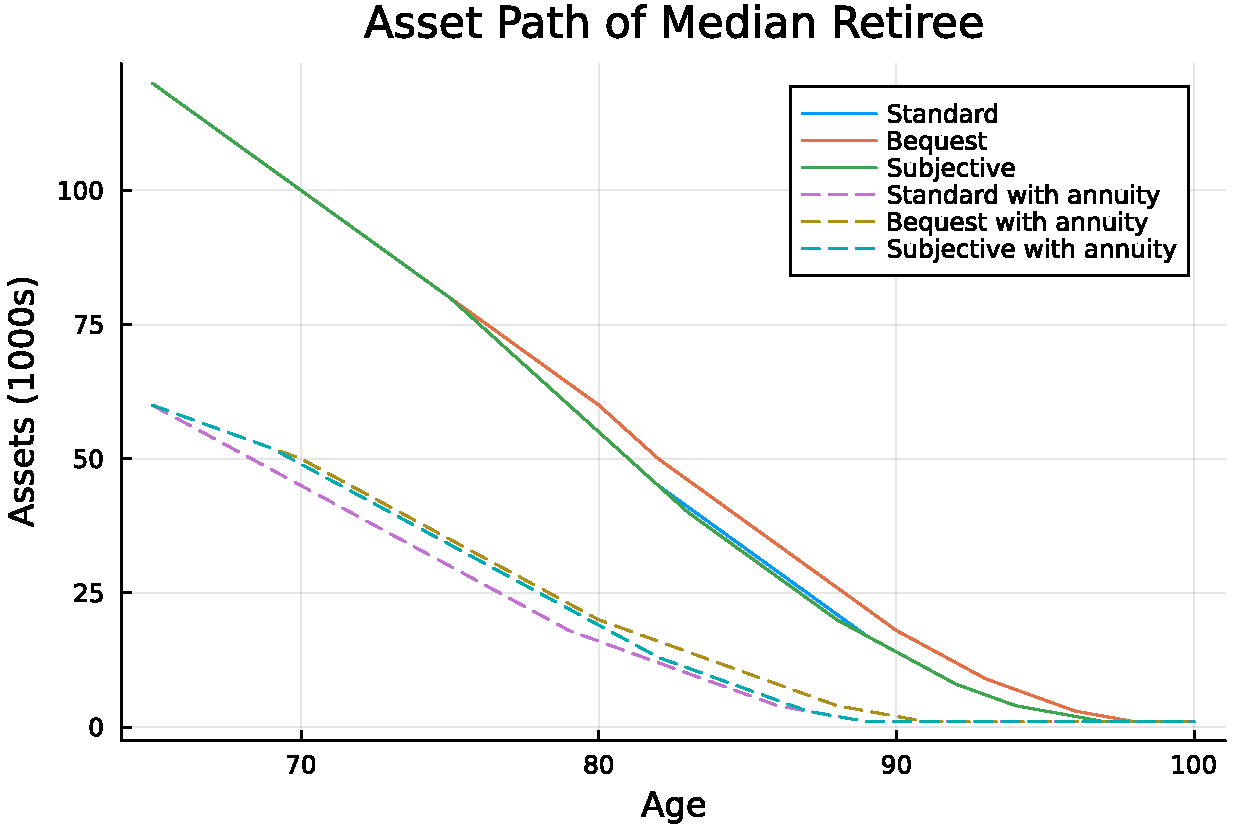
\includegraphics[width=0.7\columnwidth]{figures/asset_plot_median_retiree.pdf}
    \label{fig:AssetPlot}
\end{figure}
\begin{figure}[h]
    \caption{Consumption in retirement}
    \centering
    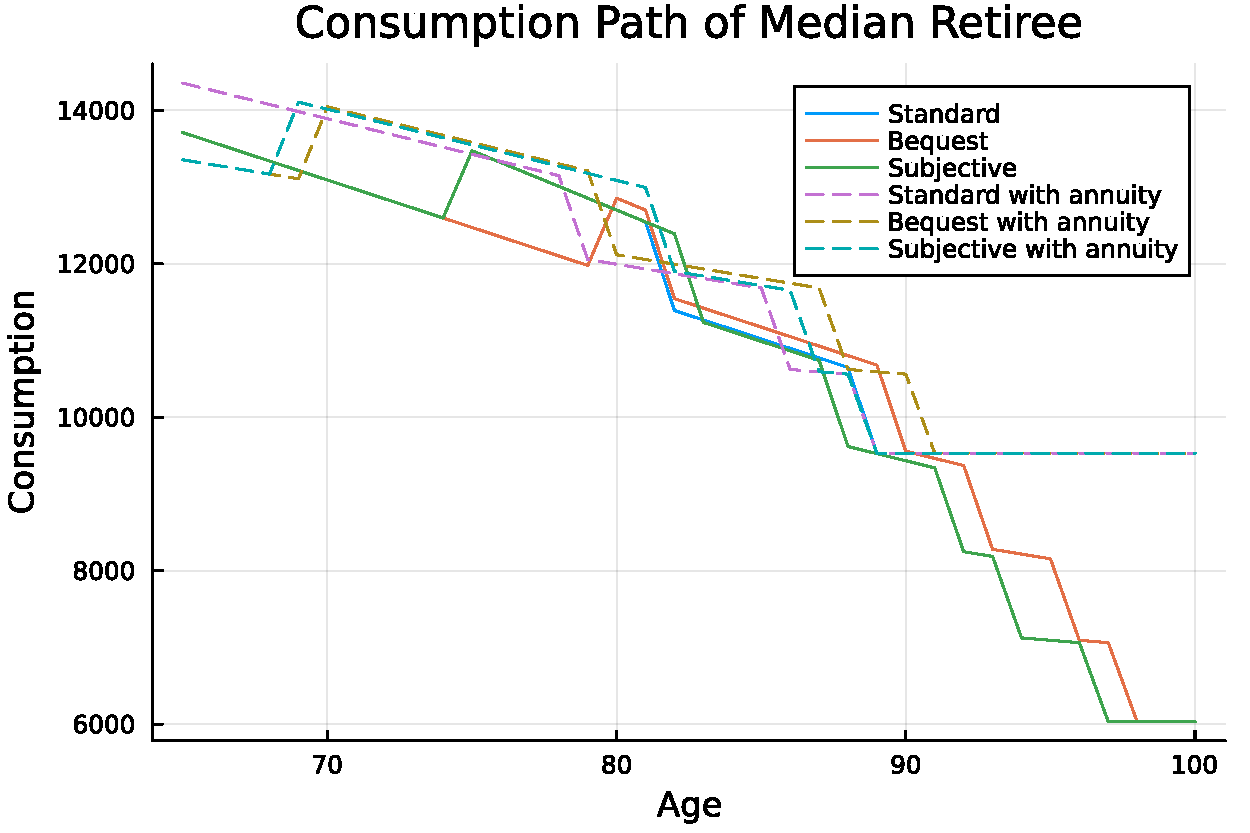
\includegraphics[width=0.7\columnwidth]{figures/consumption_plot_median_retiree.pdf}
    \label{fig:ConsumpPlot}
\end{figure}

Figures \ref{fig:AssetPlot} and \ref{fig:ConsumpPlot} show the retirement path
of consumption and assets for a median retiree. This hypothetical female has
£120,000 of assets at age 65 when she retired in 2012 with a state pension
income of £6,000. The dashed lines show consumption and assets with an annuity
that costs half of her wealth. This buys her £3,500 of annuity income, which,
given her objective life expectancy, is a money's worth of about 90\%.

We can see that the asset path with the bequest motive remains higher for longer
but still decreases, and by the woman's late 90s she has completely run down her
wealth. Interestingly, the asset path with the quickest run down is the standard
lifecycle model using objective life expectancies, which points towards this
individual being optimistic about her life chances. Also rather surprisingly,
the asset paths of all three types are similar without annuities. The paths only
diverge after age 75, at which point the bequest path stays high and the other
paths start to decrease faster. This is contrary to the path with annuities
which show the standard path diverging from the bequest and subjective paths
immediately.

The consumption paths all start at around £14,000 a year. The three models without an
annuity start at exactly the same amount and stay that way until the individual
reaches her mid seventies -- showing that even quite different lifecycle models
can generate similar paths. As expected, the consumption path with the bequest
motive with an annuity is lower at the start of retirement than the bequest path
without an annuity as individuals seek to build their savings back up. But it is
also lower for the subjective life expectancy case, again pointing toward this
individual being optimistic. However, the subjective consumption line rises at a
younger age than the line with bequests, showing that the models align with the
prediction that subjective lifecycle agents consume more in early retirement
compared to the other lifecycle models because people underpredict lifespan.

It is worth noting that the period of interest of this study is early retirement
and although differences across the lifecycle are not large, there are
significant differences at the start of retirement. This means that different
lifecycle models will produce substantive differences in predictions, so knowing
which model is correct is important for policy.

To simulate consumption and asset paths for the individuals in my ELSA dataset,
I round financial wealth and state pension income to the closest point on the
discrete asset and pension grids respectively. I then take the treatment group
and evaluate their consumption in the year of interview with an annuity, given
that they annuitised 50\% of their financial wealth in their retirement year. I
also evaluate consumption without annuitisation. The treatment group did not
need to annuitise their wealth, so I use their predicted consumption from the
lifecycle models with their starting values of assets and pension income taken
from their values in the ELSA dataset. To be clear, the only individuals for
whom I annuitise wealth are those with DC pension pots who retired before 2014.

Because I discretised the state space, annuity prices are rounded down to the
nearest income grid point. I set the money's worth of annuities to $0.9$ when
calculating annuity prices, but because I round down to the nearest income grid
point the real money's worth an individual receives is lower. I assume that
those who have a DC pension have half of their financial wealth in it since this
matches roughly what is seen in the summary statistics, so, for the untreated
group -- those who retired pre-reform -- I annuitise half of wealth. I also only
annuitise when an individual has financial assets large enough to move up at
least one unit of income (£500). I do not let these individuals, with low
assets, annuitise, setting consumption with and without an annuity to the same
amount.


\begin{table}

\caption{Model consumption predictions \label{tab:simulation_prediction}}
\centering
\begin{tabular}[t]{lrrrrrr}
\toprule
\multicolumn{1}{c}{ } & \multicolumn{2}{c}{Mean} & \multicolumn{2}{c}{Non Missing} & \multicolumn{2}{c}{Sd} \\
\cmidrule(l{3pt}r{3pt}){2-3} \cmidrule(l{3pt}r{3pt}){4-5} \cmidrule(l{3pt}r{3pt}){6-7}
 & Control & Treat & Control & Treat & Control & Treat\\
\midrule
Bequest & 891.3230 & 1041.2196 & 98 & 49 & 553.5802 & 540.8520\\
Standard & 918.5339 & 1068.4305 & 98 & 49 & 602.9341 & 573.0909\\
Subjective & 1018.3042 & 1144.9085 & 98 & 49 & 720.9637 & 597.3735\\
Total Monthly (ELSA) & 763.5413 & 887.8606 & 98 & 49 & 367.2683 & 538.9208\\
\bottomrule
\end{tabular}
\end{table}


Table \ref{tab:simulation_prediction} shows the mean of consumption that each
lifecycle model predicts for the treated and control groups as well as the
original mean of consumption from the ELSA data for the individuals with
non-missing values. The sample size of those with a DC pension is greatly
reduced. This is mainly because not everyone in the ELSA data answers the life
expectancy questions, and of those who do answer, some give answers that I
cannot use for reasons listed in the data section.

We can see that the means for the treatment group are higher than the control
for all models, but there is significant difference between the consumption
levels for the different models. The bequest and standard model both predict
lower consumption than the subjective model. This is not surprising given the
subjective lifecycle individuals generally think their lives will be shorter and
therefore can consume more early in retirement. Likewise, it makes sense that
the bequest model predicts lower consumption, since there is utility to be
gained from saving so that an individual can bequest to their heirs.


I now run the empirical models on this simulated data. This lets us see which
lifecycle model gives us the closest match to the coefficients seen in the real
data. In the structural modelling literature, it is often common to run policy
tests on estimated models to see if simulated responses match real world
responses, for example see \cite{mcgee_2021}. Due to the time constraints of
this project, I did not estimate a full structural model but I do check which
lifecycle model fits the response seen in the ELSA data.




\begin{landscape}
    \linespread{1.5}

    \begin{table}

\caption{Empirical models with simulated consumption data \label{tab:SubjectiveLifeCycle}}
\centering
\fontsize{10}{12}\selectfont
\begin{tabular}[t]{lddddddddd}
\toprule
\multicolumn{1}{c}{ } & \multicolumn{3}{c}{Bequest} & \multicolumn{3}{c}{Standard} & \multicolumn{3}{c}{Subjective} \\
\cmidrule(l{3pt}r{3pt}){2-4} \cmidrule(l{3pt}r{3pt}){5-7} \cmidrule(l{3pt}r{3pt}){8-10}
  & {DCOnly} & {DCInt} & {FinInt} & {DCOnly } & {DCInt } & {FinInt } & {DCOnly  } & {DCInt  } & {FinInt  }\\
\midrule
(Intercept) & -447.67 & -543.51 & -439.95 & -681.17 & -648.12 & -588.16 & -1026.68 & -779.75 & -1031.89\\
PostReform & 16.69 & -10.85 & 24.81 & 2.84 & -4.68 & 30.65 & -62.88 & -14.69 & 63.14\\
RetiredAge & 7.58 & 9.15 & 7.45 & 10.69 & 10.33 & 9.09 & 16.56 & 12.67 & 16.39\\
FinWealth(£000s) & 4.08 & 4.07 & 4.10 & 4.43 & 4.32 & 4.51 & 5.05 & 4.75 & 5.43\\
Gender & 13.73 & 19.65 & 13.38 & 13.07 & 23.30 & 14.34 & -62.50 & -30.43 & -52.37\\
DCValue(£000s) & 0.00 & 0.00 & {} & 0.00 & 0.00 & {} & 0.00 & 0.01 & {}\\
YearsSinceRetirement & -1.22 & -0.89 & -2.27 & -6.22 & -0.62 & -7.27 & -33.07 & 1.92 & -42.02\\
OwnsHouse & 5.06 & 17.85 & 3.84 & 14.67 & 21.49 & 13.22 & 66.45 & 44.94 & 51.10\\
StatePension & 84.42 & 84.99 & 84.40 & 89.06 & 89.24 & 89.27 & 92.85 & 92.99 & 91.54\\
DCPension & {} & -20.63 & {} & {} & -15.38 & {} & {} & 7.56 & {}\\
DBPension & {} & 0.56 & {} & {} & 1.52 & {} & {} & -13.52 & {}\\
PostReform:DCPension & {} & 25.53 & {} & {} & 17.76 & {} & {} & -30.89 & {}\\
PostReform:DBPension & {} & 2.66 & {} & {} & -11.35 & {} & {} & 16.74 & {}\\
PostReform:FinWealth(£000s) & {} & {} & -0.06 & {} & {} & -0.22 & {} & {} & -0.95\\
\midrule
Num.Obs. & 139 & 584 & 147 & 139 & 584 & 147 & 139 & 584 & 147\\
R2 & 0.996 & 0.995 & 0.996 & 0.995 & 0.993 & 0.995 & 0.961 & 0.943 & 0.966\\
R2 Adj. & 0.995 & 0.995 & 0.995 & 0.994 & 0.993 & 0.995 & 0.958 & 0.942 & 0.964\\
\bottomrule
\end{tabular}
\end{table}

\end{landscape}


Table \ref{tab:SubjectiveLifeCycle} shows all these results. Each set of colums shows the
results from the empirical models using a different lifecycle model to simulate
the data. The sub columns show the empirical modes: the first runs the
regression discontinuity just on those with DC pensions, the second looks at
all individuals and uses the DD set up, whilst the third interacts financial
wealth with the treatment indicator for those with DC pensions only.

Comparing the DC-only column across lifecycle models, we can see that the
simulated bequest model gives us the highest increase in consumption as a result
of forced annuitisation. This could be because this type of individual was
previously saving out of their annuity income to regain assets, so when they do
not need to buy an annuity anymore their consumption increases. Surprisingly,
when using the predictions from subjective models, the coefficient on PostReform
is negative, even though the mean increased for this model as shown in Table
\ref{tab:simulation_prediction}.

The lifecycle model that is closest to the empirical models shown in Table
\ref{tab:DcOnlyRes} is the bequest model which gives an increase of 17 in
monthly consumption. However, this coefficient is just under half of the change
estimated in Table \ref{tab:DcOnlyRes} and reflects only a 0.6\% rise in
consumption after the reform.

In the second column, the coefficient of interest is the DC pension interaction
with the treatment variable since I use the DD setup again. The bequest model
has a coefficient of 25.5, the standard model one of 17.8 and the standard model
with subjective life expectancies has one of -30.9. The bequest and subjective
coefficients are higher than the coefficient seen in Table \ref{tab:ElsaAllData}
with the predictions from the standard model matching the empirical model best.
The subjective model again has the opposite sign to the one seen in the
empirical model.

The interaction model in column 3 has the sign for the main
reform effect in the standard and bequest models. Although in both the
interaction with financial wealth has a negative coefficient, showing that the
increase in consumption caused by the reform was progressively lower for those
who would have had to annuitise more wealth. In the subjective model table, the
signs are again wrong apart from for the main treatment effect in the financial
interaction column. The lifecycle model that appears closest to the empirical
results is again the bequest model, which matches the signs from Tables
\ref{tab:DcOnlyInteract} and \ref{tab:DcOnlyFinWealthInteract}, but the
coefficients are smaller.

Across all regressions, the lifecycle model using subjective life expectancies
does not match the change in consumption that is seen when using ELSA data. It
is surprising that the consumption response is also very different to the other
lifecycle models used. One possible explanation for this could be that the
control and treatment groups have quite different sets of subjective life
expectancies, which therefore cause different consumption paths in early
retirement. This heterogeneity in death probabilities would not occur in the
other models because the difference in objective death probabilities at a given
age for different birth cohorts is not that large, whereas differences in
subjective life expectancies between individuals can be big. The structure that
the Weibull distribution imposes on the death probabilities could also be
causing discontinuities in a given individuals subjective probability of death
between two periods, which would impact how they consume across that part of
retirement.

The evidence just presented points towards data simulated using the bequest
model being best able to replicate the consumption response observed in the
empirical models. As highlighted above, the benefit of having a theoretical
model is that we can trace out the asset path of consumption for individuals,
only needing to know their retirement wealth as we were able to do in
Figure \ref{fig:AssetPlot}.

\section{Conclusion}

The results from the empirical section of this paper point towards there being
some impact of the UK's pensions freedom act on the consumption of retirees
early in retirement. The specifications that used the full available dataset
show a clear increase in total monthly consumption, and particularly an increase
in food consumption away from home and on spending on clothes. Although the
increase of £36 in total monthly consumption only equates to £432 a year, over
a longer period it may mean some retirees end up with fewer resources than they
require toward the end of their life.

Moreover, the results from the lifecycle section show not just that the models
create different consumption predictions, but they also add to the evidence that
lifecycle models with bequests can do a good job of explaining the consumption
patterns of retirees in the UK. That simulated data from a bequest model matches
the consumption response also points towards bequests being able to explain the
annuitisation puzzle.

Since the bequest motive model fits the consumption response best, we can worry
about the increase in early retirement consumption less. This is because, as
highlighted in the analysis of the median individual, assets in the bequest model
diverge from the objective and subjective lifecycle models during retirement,
reducing at a slower rate. Therefore, the government should not worry about
spending early in retirement being linked to low assets at the end of an
individual's life. The bequest explanation also has implications for the
macroeconomic impact of other public policy --- for example it means an
inheritance tax could impact the savings of retirees.

Future research is still needed to understand the full impact the reform has had
on consumption across the whole of retirement, especially as more data on
retirees impacted by the reform becomes available. The effect that reforms since
this one, such as allowing individuals on DB plans to switch to DC plans, has
had on consumption could also be studied. Moreover, as the number of individuals
retiring with a DC pension grows, understanding the mechanisms
behind their choices will matter more to policy makers. For example, if the
annuitisation puzzle is caused by a bequest motive rather than low money's worth
or short subjective life expectancies, then policies that force annuitisation or
tax assets to fund state pensions will not be welfare-enhancing.




\bibliographystyle{apa}
\bibliography{references}
\end{document}